\documentclass[aspectratio=169]{beamer}
\usetheme{Madrid}
\usecolortheme{crane}

\usepackage[utf8]{inputenc}
\usepackage[T1]{fontenc}
\usepackage{booktabs}
\usepackage{tikz}
\usetikzlibrary{shapes.geometric, arrows.meta, positioning, fit, backgrounds}

% Custom colors
\definecolor{natoblue}{RGB}{0, 57, 107}
\definecolor{natowhite}{RGB}{255, 255, 255}
\definecolor{critical}{RGB}{180, 30, 30}
\definecolor{high}{RGB}{220, 120, 20}
\definecolor{medium}{RGB}{200, 180, 40}

\setbeamercolor{palette primary}{bg=natoblue, fg=natowhite}
\setbeamercolor{palette secondary}{bg=natoblue!80, fg=natowhite}
\setbeamercolor{palette tertiary}{bg=natoblue!60, fg=natowhite}
\setbeamercolor{title}{fg=natoblue}
\setbeamercolor{frametitle}{fg=natoblue}
\setbeamercolor{block title}{bg=natoblue, fg=natowhite}
\setbeamercolor{block body}{bg=natoblue!5}

\setbeamertemplate{navigation symbols}{}
\setbeamertemplate{footline}[frame number]

\title{\textbf{NATO Smart City IoT}}
\subtitle{Automated Attack Path Analysis Platform -- Q1 2026}
\author{T. Vansnick, M. Delehouzée, I. Hentous, S. Mahmoudi}
\institute{University of Mons}
\date{March 2026}

\begin{document}

% =============================================
% SLIDE 1: Title
% =============================================
\begin{frame}
\titlepage
\end{frame}

% =============================================
% SLIDE 2: Physical Lab
% =============================================
\begin{frame}{Physical Lab Infrastructure}

\begin{columns}[T]
\begin{column}{0.5\textwidth}
\textbf{192.xxx.x.0/24} -- Real devices, real vulnerabilities

\vspace{0.3cm}
\small
\begin{tabular}{ll}
\toprule
\textbf{Category} & \textbf{Devices} \\
\midrule
Router & MikroTik RB5009 \\
Switch & Netgear GS348PP (PoE) \\
Gateways & RPi5, WisGate, IoT Hub \\
Compute & Jetson Orin Nano \\
Sensors & 4x LoRaWAN, 2x Zigbee \\
Camera & Ubiquiti AI Turret \\
WiFi AP & TP-Link EAP613 \\
\midrule
\textbf{Total} & \textbf{15 devices, 16 links} \\
\bottomrule
\end{tabular}

\vspace{0.3cm}
\small 5 protocols -- 20 open services -- 24 known CVEs
\end{column}

\begin{column}{0.48\textwidth}
\centering
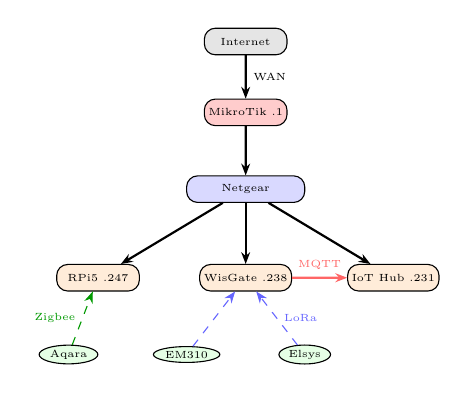
\begin{tikzpicture}[
    d/.style={rectangle, draw, rounded corners, minimum width=1.4cm, minimum height=0.45cm, font=\tiny, inner sep=2pt},
    s/.style={ellipse, draw, font=\tiny, inner sep=1pt, fill=green!10},
    a/.style={-{Stealth[length=1.5mm]}, thick},
    w/.style={-{Stealth[length=1.5mm]}, dashed},
    scale=0.75, transform shape,
]
\node[d, fill=gray!20] (inet) at (0,5.5) {Internet};
\node[d, fill=red!20] (mk) at (0,4.3) {MikroTik .1};
\node[d, fill=blue!15, minimum width=2cm] (ng) at (0,3) {Netgear};

\node[d, fill=orange!15] (rpi) at (-2.5,1.5) {RPi5 .247};
\node[d, fill=orange!15] (wg) at (0,1.5) {WisGate .238};
\node[d, fill=orange!15] (hub) at (2.5,1.5) {IoT Hub .231};

\node[s] (a1) at (-3,0.2) {Aqara};
\node[s] (e1) at (-1,0.2) {EM310};
\node[s] (e2) at (1,0.2) {Elsys};

\draw[a] (inet) -- (mk) node[midway, right, font=\tiny] {WAN};
\draw[a] (mk) -- (ng);
\draw[a] (ng) -- (rpi);
\draw[a] (ng) -- (wg);
\draw[a] (ng) -- (hub);
\draw[w, green!60!black] (a1) -- (rpi) node[midway, left, font=\tiny] {Zigbee};
\draw[w, blue!60] (e1) -- (wg);
\draw[w, blue!60] (e2) -- (wg) node[midway, right, font=\tiny] {LoRa};
\draw[a, red!60] (wg) -- (hub) node[midway, above, font=\tiny] {MQTT};
\end{tikzpicture}
\end{column}
\end{columns}
\end{frame}

% =============================================
% SLIDE 4: Evolution Q4 -> Q1
% =============================================
\begin{frame}{Evolution: Q4 2025 $\rightarrow$ Q1 2026}

\begin{table}
\centering
\small
\begin{tabular}{@{}lll@{}}
\toprule
\textbf{Component} & \textbf{Q4 2025} & \textbf{Q1 2026} \\
\midrule
Infrastructure & JSON (simulated) & \textbf{YAML} (real lab) \\
Graph DB & Neo4j (external) & \textbf{NetworkX} (in-process) \\
Cache & MongoDB & \textbf{ChromaDB} (vector search) \\
AI & MCP + Ollama (single query) & \textbf{5-phase agent pipeline} \\
Attack paths & Basic traversal & \textbf{Dijkstra-weighted} \\
Tools & Hardcoded Python & \textbf{Declarative YAML} (9 tools) \\
Risk scoring & CVSS only & \textbf{CVSS + centrality + hops} \\
Tests & Manual & \textbf{193 automated tests} \\
\bottomrule
\end{tabular}
\end{table}

\vspace{0.3cm}
\begin{block}{Key rationale}
Neo4j $\rightarrow$ NetworkX: 15 nodes don't need an external DB. Abstract \texttt{GraphBackend} ABC allows swapping to Neo4j/Memgraph for \textbf{real smart city scale} (1000+ devices). \quad MongoDB $\rightarrow$ ChromaDB: enables \textbf{semantic search}. \quad MCP $\rightarrow$ Pipeline: enables \textbf{multi-step reasoning}.
\end{block}
\end{frame}

% =============================================
% SLIDE 5: Architecture
% =============================================
\begin{frame}{Platform Architecture}

\centering
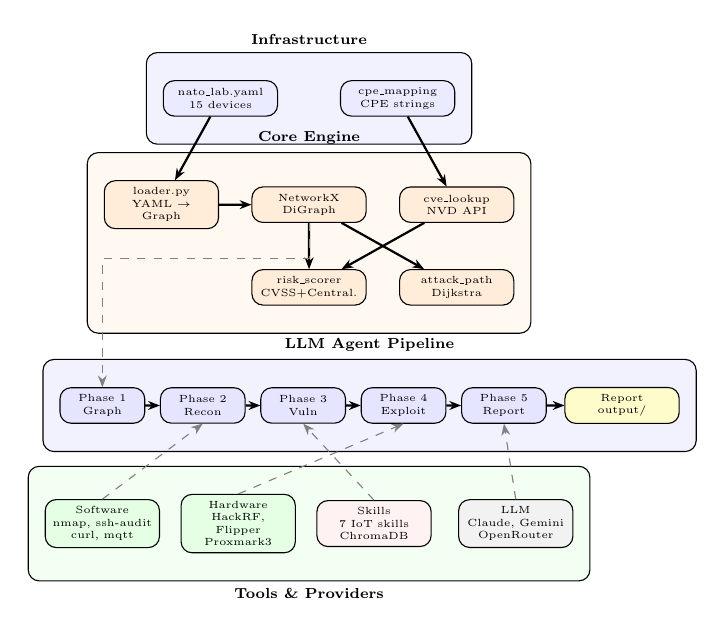
\begin{tikzpicture}[
    b/.style={rectangle, draw, rounded corners, minimum width=1.8cm, minimum height=0.6cm, font=\tiny, text width=1.7cm, align=center},
    p/.style={rectangle, draw, rounded corners, minimum width=1.3cm, minimum height=0.6cm, font=\tiny, text width=1.2cm, align=center, fill=blue!10},
    g/.style={rectangle, draw, rounded corners, inner sep=6pt, inner ysep=10pt},
    a/.style={-{Stealth[length=1.5mm]}, thick},
    d/.style={-{Stealth[length=1.5mm]}, dashed, gray},
    scale=0.75, transform shape,
]

% Infrastructure
\node[b, fill=blue!8] (yaml) at (0,0) {nato\_lab.yaml\\15 devices};
\node[b, fill=blue!8] (cpe) at (3,0) {cpe\_mapping\\CPE strings};

% Core
\node[b, fill=orange!15] (loader) at (-1, -1.8) {loader.py\\YAML $\rightarrow$ Graph};
\node[b, fill=orange!15] (graph) at (1.5, -1.8) {NetworkX\\DiGraph};
\node[b, fill=orange!15] (cve) at (4, -1.8) {cve\_lookup\\NVD API};
\node[b, fill=orange!15] (risk) at (1.5, -3.2) {risk\_scorer\\CVSS+Central.};
\node[b, fill=orange!15] (attack) at (4, -3.2) {attack\_path\\Dijkstra};

% Pipeline
\node[p] (p1) at (-2, -5.2) {Phase 1\\Graph};
\node[p] (p2) at (-0.3, -5.2) {Phase 2\\Recon};
\node[p] (p3) at (1.4, -5.2) {Phase 3\\Vuln};
\node[p] (p4) at (3.1, -5.2) {Phase 4\\Exploit};
\node[p] (p5) at (4.8, -5.2) {Phase 5\\Report};
\node[b, fill=yellow!20] (out) at (6.8, -5.2) {Report\\output/};

% Tools
\node[b, fill=green!10] (sw) at (-2, -7.2) {Software\\nmap, ssh-audit\\curl, mqtt};
\node[b, fill=green!10] (hw) at (0.3, -7.2) {Hardware\\HackRF, Flipper\\Proxmark3};
\node[b, fill=pink!20] (sk) at (2.6, -7.2) {Skills\\7 IoT skills\\ChromaDB};
\node[b, fill=gray!10] (llm) at (5, -7.2) {LLM\\Claude, Gemini\\OpenRouter};

% Arrows
\draw[a] (yaml) -- (loader);
\draw[a] (cpe) -- (cve);
\draw[a] (loader) -- (graph);
\draw[a] (graph) -- (risk);
\draw[a] (cve) -- (risk);
\draw[a] (graph) -- (attack);

\draw[a,thick] (p1) -- (p2);
\draw[a,thick] (p2) -- (p3);
\draw[a,thick] (p3) -- (p4);
\draw[a,thick] (p4) -- (p5);
\draw[a] (p5) -- (out);

\draw[d] (sw.north) -- (p2.south);
\draw[d] (hw.north) -- (p4.south);
\draw[d] (sk.north) -- (p3.south);
\draw[d] (llm.north) -- (p5.south);
\draw[d] (graph.south) -- ++(0,-0.6) -| (p1.north);

% Groups
\begin{scope}[on background layer]
    \node[g, fill=blue!5, fit=(yaml)(cpe), label={[font=\scriptsize\bfseries]above:Infrastructure}] {};
    \node[g, fill=orange!5, fit=(loader)(graph)(cve)(risk)(attack), label={[font=\scriptsize\bfseries]above:Core Engine}] {};
    \node[g, fill=blue!5, fit=(p1)(p2)(p3)(p4)(p5)(out), label={[font=\scriptsize\bfseries]above:LLM Agent Pipeline}] {};
    \node[g, fill=green!5, fit=(sw)(hw)(sk)(llm), label={[font=\scriptsize\bfseries]below:Tools \& Providers}] {};
\end{scope}
\end{tikzpicture}
\end{frame}

% =============================================
% SLIDE 6: Agent Pipeline
% =============================================
\begin{frame}{LLM Agent Pipeline: 5 Phases}

\begin{table}
\centering
\small
\begin{tabular}{@{}clllc@{}}
\toprule
\textbf{\#} & \textbf{Agent} & \textbf{Tools} & \textbf{Output} & \textbf{Turns} \\
\midrule
1 & Graph Analysis & graph queries & Topology + attack surface & 3 \\
2 & Reconnaissance & nmap, ssh-audit, curl, mqtt & Confirmed services & 9 \\
3 & Vuln Analysis & recon + NVD + skills & Per-device CVE analysis & 34 \\
4 & Exploitation & recon + hardware & Exploit validation & -- \\
5 & Report & graph + deliverables & Final pentest report & 4 \\
\bottomrule
\end{tabular}
\end{table}

\vspace{0.3cm}
\begin{columns}[T]
\begin{column}{0.48\textwidth}
\begin{block}{Agentic loop}
\begin{enumerate}
    \item Agent receives system prompt
    \item Calls tools (nmap, mqtt\_listen...)
    \item Analyzes results
    \item Iterates until deliverable is ready
    \item Saves deliverable for next phase
\end{enumerate}
\end{block}
\end{column}
\begin{column}{0.48\textwidth}
\begin{block}{Phase 3: Per-device sub-agents}
\begin{itemize}
    \item Spawns one agent per attack surface device
    \item MikroTik, WisGate, RPi5, IoT Hub, Jetson, EAP613
    \item Parallelized vulnerability analysis
    \item Each produces a JSON vulnerability report
\end{itemize}
\end{block}
\end{column}
\end{columns}
\end{frame}

% =============================================
% SLIDE 7: Tool System
% =============================================
\begin{frame}{Declarative Tool System}

\begin{columns}[T]
\begin{column}{0.48\textwidth}
\begin{block}{Software tools (5) -- auto-executed}
\small
\begin{itemize}
    \item \texttt{nmap\_scan} -- Service detection
    \item \texttt{ssh\_audit} -- SSH config analysis
    \item \texttt{curl\_headers} -- HTTP headers
    \item \texttt{mqtt\_listen} -- MQTT sniffing
    \item \texttt{nvd\_lookup} -- CVE search
\end{itemize}
\end{block}

\vspace{0.2cm}
\begin{alertblock}{Adding a new tool}
\small
Just create a YAML file in \texttt{definitions/}\\
No Python code needed!
\end{alertblock}
\end{column}

\begin{column}{0.48\textwidth}
\begin{block}{Hardware tools (4) -- operator-guided}
\small
\begin{itemize}
    \item \texttt{hackrf\_capture} -- SDR 1--6 GHz
    \item \texttt{flipper\_zero} -- Multi-protocol
    \item \texttt{proxmark3} -- RFID/NFC cracking
    \item \texttt{exploit\_iot\_kit} -- UART/JTAG/SPI
\end{itemize}
\end{block}

\vspace{0.2cm}
\begin{exampleblock}{How hardware tools work}
\small
Agent calls \texttt{hackrf\_capture(zigbee)}\\
$\rightarrow$ Returns specific commands\\
$\rightarrow$ Operator executes on hardware\\
$\rightarrow$ Results feed back to agent
\end{exampleblock}
\end{column}
\end{columns}
\end{frame}

% =============================================
% SLIDE 8: Hardware Attack Tools
% =============================================
\begin{frame}{Hardware Attack Tools}

\begin{table}
\centering
\small
\begin{tabular}{@{}llp{7cm}@{}}
\toprule
\textbf{Tool} & \textbf{Type} & \textbf{Lab applications} \\
\midrule
\textbf{HackRF One} & SDR & Zigbee 802.15.4 sniffing (2.4 GHz channels 11--26), LoRaWAN EU868 capture, GNU Radio decoding \\
\textbf{Flipper Zero} & Multi-tool & Sub-GHz replay, RFID/NFC emulation, GPIO/UART bridging to devices \\
\textbf{Proxmark3 Easy} & RFID/NFC & Mifare Classic cracking (darkside, hardnested), badge cloning for physical access \\
\textbf{Exploit IoT Kit} & HW hacking & UART console on WisGate, JTAG debug on sensors, SPI flash dump, firmware extraction \\
\bottomrule
\end{tabular}
\end{table}

\vspace{0.3cm}
\begin{block}{Integration approach (OWASP ISTG + PTES hybrid)}
\begin{itemize}
    \item Declarative YAML definitions with \texttt{type: hardware} marker
    \item Protocol-specific commands per tool (Zigbee, LoRaWAN, NFC, UART...)
    \item Skills cross-reference hardware: \texttt{zigbee\_security.md} $\rightarrow$ \texttt{tools: [hackrf\_capture]}
    \item Agent recommends commands; operator executes with physical access
\end{itemize}
\end{block}
\end{frame}

% =============================================
% SLIDE 9: Knowledge Store
% =============================================
\begin{frame}{Knowledge Store: Skills + ChromaDB}

\begin{columns}[T]
\begin{column}{0.45\textwidth}
\begin{block}{7 IoT Security Skills}
\footnotesize
\begin{tabular}{ll}
\toprule
\textbf{Skill} & \textbf{Focus} \\
\midrule
mqtt\_security & Anonymous access \\
zigbee\_security & RF + key extraction \\
lorawan\_analysis & ABP replay \\
firmware\_analysis & Flash dump, UART \\
ssh\_hardening & Terrapin, ciphers \\
mikrotik\_routeros & RouterOS CVEs \\
web\_service & HTTP headers \\
\bottomrule
\end{tabular}
\end{block}

\vspace{0.1cm}
\begin{exampleblock}{Semantic search}
\footnotesize
``UART firmware dump'' $\rightarrow$ firmware\_analysis [0.68]\\
``MQTT anonymous'' $\rightarrow$ mqtt\_security [0.63]
\end{exampleblock}
\end{column}

\begin{column}{0.52\textwidth}
\begin{block}{RAG pipeline}
\footnotesize
\begin{enumerate}
    \item Markdown skills with YAML frontmatter (name, tags, tools)
    \item Chunked by \texttt{\#\#} headings with context prefix
    \item Embedded via Voyage AI (512 dims)
    \item Stored in ChromaDB (46 chunks, persistent)
    \item Agent calls \texttt{search\_knowledge(query)}
    \item Top-k chunks returned by cosine similarity
\end{enumerate}
\end{block}

\vspace{0.1cm}
\begin{block}{Benefits}
\footnotesize
\begin{itemize}
    \item No full skill in prompt $\rightarrow$ context window savings
    \item Fuzzy matching (no exact keywords needed)
    \item New skills auto-searchable after ingestion
\end{itemize}
\end{block}
\end{column}
\end{columns}
\end{frame}

% =============================================
% SLIDE 10: Results - Metrics
% =============================================
\begin{frame}{Results: Pipeline Execution}

\begin{columns}[T]
\begin{column}{0.55\textwidth}
\begin{table}
\centering
\small
\begin{tabular}{@{}lccc@{}}
\toprule
\textbf{Phase} & \textbf{Turns} & \textbf{Cost} & \textbf{Time} \\
\midrule
Graph Analysis & 3 & \$0.01 & 16s \\
Reconnaissance & 9 & \$0.17 & 11m \\
Vuln Analysis & 34 & \$0.18 & 11m \\
Report & 4 & \$0.02 & 18s \\
\midrule
\textbf{Total} & \textbf{50} & \textbf{\$0.38} & \textbf{23m} \\
\bottomrule
\end{tabular}
\caption*{\small Gemini 3 Flash Preview -- March 16, 2026}
\end{table}
\end{column}

\begin{column}{0.4\textwidth}
\begin{block}{Key metrics}
\begin{itemize}
    \item 99 tool calls
    \item 674K input tokens
    \item 6 devices scanned
    \item 5 vulnerabilities found
    \item 2 attack paths identified
\end{itemize}
\end{block}

\vspace{0.2cm}
\textbf{Cost:} \$0.38 per full assessment\\
\textbf{vs.} Nessus: \$5K+/year license
\end{column}
\end{columns}
\end{frame}

% =============================================
% SLIDE 11: Results - Findings
% =============================================
\begin{frame}{Results: Discovered Vulnerabilities}

\begin{table}
\centering
\small
\begin{tabular}{@{}llll@{}}
\toprule
\textbf{Finding} & \textbf{Device} & \textbf{Service} & \textbf{Severity} \\
\midrule
\textcolor{critical}{\textbf{Anonymous MQTT access}} & RPi5 & Mosquitto 1883 & \textcolor{critical}{\textbf{CRITICAL}} \\
CVE-2023-51767 (DoS) & RPi5 / IoT Hub & Mosquitto & \textcolor{high}{\textbf{HIGH}} \\
CVE-2021-23017 (RCE) & WisGate & nginx 1.19.6 & \textcolor{high}{\textbf{HIGH}} \\
CVE-2021-3014 (DNS) & MikroTik & RouterOS & \textcolor{medium}{\textbf{MEDIUM}} \\
CVE-2019-9511 (DoS) & Jetson & HTTP/2 & \textcolor{medium}{\textbf{MEDIUM}} \\
\bottomrule
\end{tabular}
\end{table}

\vspace{0.3cm}
\begin{alertblock}{Critical finding: Anonymous MQTT}
\begin{itemize}
    \item Agent ran \texttt{mqtt\_listen(broker="192.xxx.x.247")} and received live Zigbee sensor data
    \item \textbf{No credentials required} -- anyone on the LAN can intercept all smart city data
    \item Aqara vibration + door sensors data exposed (occupancy patterns = behavioral PII)
\end{itemize}
\end{alertblock}
\end{frame}

% =============================================
% SLIDE 12: Attack Paths
% =============================================
\begin{frame}{Attack Paths: Multi-Hop Chains}

\begin{block}{Path 1: Data Exfiltration}
\centering
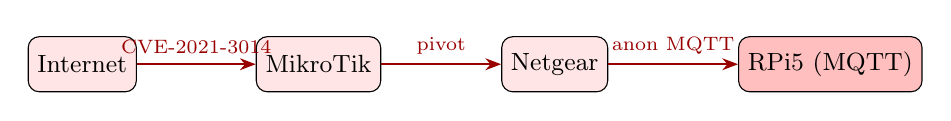
\begin{tikzpicture}[
    n/.style={rectangle, draw, rounded corners, fill=red!10, font=\small, minimum height=0.7cm},
    a/.style={-{Stealth[length=2mm]}, thick, red!60!black},
]
\node[n] (i) at (0,0) {Internet};
\node[n] (mk) at (3,0) {MikroTik};
\node[n] (ng) at (6,0) {Netgear};
\node[n, fill=red!25] (rpi) at (9.5,0) {RPi5 (MQTT)};
\draw[a] (i) -- (mk) node[midway, above, font=\scriptsize] {CVE-2021-3014};
\draw[a] (mk) -- (ng) node[midway, above, font=\scriptsize] {pivot};
\draw[a] (ng) -- (rpi) node[midway, above, font=\scriptsize] {anon MQTT};
\end{tikzpicture}
\end{block}

\vspace{0.3cm}
\begin{block}{Path 2: Infrastructure Takeover}
\centering
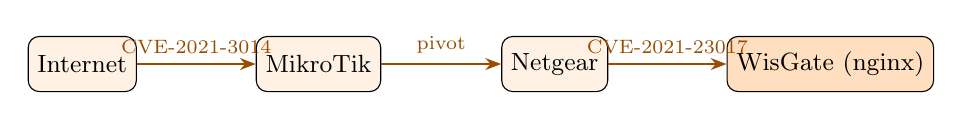
\begin{tikzpicture}[
    n/.style={rectangle, draw, rounded corners, fill=orange!10, font=\small, minimum height=0.7cm},
    a/.style={-{Stealth[length=2mm]}, thick, orange!60!black},
]
\node[n] (i) at (0,0) {Internet};
\node[n] (mk) at (3,0) {MikroTik};
\node[n] (ng) at (6,0) {Netgear};
\node[n, fill=orange!25] (wg) at (9.5,0) {WisGate (nginx)};
\draw[a] (i) -- (mk) node[midway, above, font=\scriptsize] {CVE-2021-3014};
\draw[a] (mk) -- (ng) node[midway, above, font=\scriptsize] {pivot};
\draw[a] (ng) -- (wg) node[midway, above, font=\scriptsize] {CVE-2021-23017};
\end{tikzpicture}
\end{block}

\vspace{0.3cm}
\centering
\small\textit{Graph-based analysis reveals compound risks invisible to device-centric scanners}
\end{frame}

% =============================================
% SLIDE 13: Risk Scores
% =============================================
\begin{frame}{Risk Scoring}

\begin{columns}[T]
\begin{column}{0.48\textwidth}
\begin{block}{Formula}
$\text{Score} = \prod P(\text{hop}_i) \times \text{impact} \times \text{amplification}^{n-1}$
\end{block}

\vspace{0.2cm}
\textbf{Three factors:}
\begin{itemize}
    \item CVSS maximum (vulnerability severity)
    \item Betweenness centrality (pivot importance)
    \item Hop distance from Internet
\end{itemize}

\vspace{0.2cm}
\textbf{Protocol factors:}\\
Ethernet 1.0, WiFi 0.9, MQTT 0.8,\\
LoRaWAN 0.6, Zigbee 0.5
\end{column}

\begin{column}{0.48\textwidth}
\begin{table}
\centering
\small
\begin{tabular}{@{}lccc@{}}
\toprule
\textbf{Device} & \textbf{Risk} & \textbf{CVSS} & \textbf{Central.} \\
\midrule
mikrotik & \textbf{6.6} & 7.5 & 0.13 \\
wisgate & \textbf{5.6} & 7.7 & 0.47 \\
rpi5 & \textbf{5.3} & 9.3 & 0.25 \\
iot\_hub & 4.1 & 9.3 & 0.00 \\
netgear & 3.0 & 0.0 & \textbf{0.72} \\
\bottomrule
\end{tabular}
\end{table}

\begin{exampleblock}{Insight}
\small Netgear has no CVEs but risk=3.0 due to \textbf{highest centrality} (0.72) -- it's the network nexus
\end{exampleblock}
\end{column}
\end{columns}
\end{frame}

% =============================================
% SLIDE 14: Next Steps
% =============================================
\begin{frame}{Next Steps: Q2 2026}

\begin{columns}[T]
\begin{column}{0.48\textwidth}
\begin{block}{Progressive Pentesting}
\begin{enumerate}
    \item \textbf{Safe tests} on real lab
    \begin{itemize}
        \small
        \item MQTT anonymous access
        \item SSH default credentials
        \item Terrapin scan
    \end{itemize}
    \item \textbf{Destructive tests} on Docker
    \begin{itemize}
        \small
        \item nginx:1.19.6 exploits
        \item Dropbear 2020.81
        \item MikroTik CHR
    \end{itemize}
\end{enumerate}
\end{block}
\end{column}

\begin{column}{0.48\textwidth}
\begin{block}{New capabilities}
\begin{itemize}
    \item \textbf{NFC access control}: PN532 reader on RPi + Proxmark3 badge cloning
    \item \textbf{RF testing}: HackRF Zigbee sniffing (ch 11--26) + LoRaWAN EU868 capture
    \item \textbf{Firmware extraction}: UART/JTAG on WisGate via exploit kit
    \item \textbf{End-to-end chains}: combine network + RF + physical vectors
\end{itemize}
\end{block}
\end{column}
\end{columns}
\end{frame}

\end{document}
